\chapter{Bilan de masse: annexes}
\section{Flowsheet}\label{appendix:flowsheet}

\tikzstyle{decision} = [diamond, draw, fill=blue!20,
    text width=4.5em, text badly centered, node distance=3cm, inner sep=0pt]
\tikzstyle{block} = [rectangle, draw, fill=blue!20,
    text width=14em, text centered, rounded corners, minimum height=4em, minimum width=15em, node distance=3cm]
\tikzstyle{block2} = [rectangle, draw, fill=red!20,
    text width=14em, text centered, rounded corners, minimum height=4em, minimum width=15em, node distance=3cm]
\tikzstyle{line} = [draw, -latex']
\tikzstyle{cloud} = [draw, ellipse,fill=red!20, node distance=3cm,
    minimum height=2em]

\begin{figure}
	\begin{tikzpicture}[node distance = 3cm, auto]
	    % Place nodes
	    \node [block] (RefPrim) {\textbf{Réformage primaire}(Réformage à vapeur de \ce{CH_4}) $$\ce{CH_4 + H_2O \Leftrightarrow CO + 3H_2}$$ \textit{Equilibre à T (sortie)} };
	    \node [block2, left of=RefPrim, node distance=7cm] (Four) {\textbf{Four} \\ Combustion de \ce{CH_4} \\ \textit{Irreversible et complète}};
	    \node [block, below of=RefPrim, node distance=3.5cm] (RefSec) {\textbf{Réformage secondaire} $$\ce{2CH_2 + O_2 \Rightarrow}$$ \textit{Considérée comme irréversible et complète à la fin.}};
	    \node [block, below of=RefSec, node distance=3.5cm] (Reacteur) {\textbf{Réacteurs Water-Gas-Shift} $$\ce{CO + H_2O \Rightarrow CO_2 + H_2}$$ \textit{Considérée comme complète à la fin.} };
	    \node [block, below of=Reacteur, node distance=3.5cm] (AbsComp) {\textbf{Absorption de \ce{CO_2} et compression} (séparation d'\ce{H_2 O}) \\ \textit{Considérées complètes.}};
	    \node [block, below of=AbsComp, node distance=3.5cm] (Synth) {\textbf{Synthèse d'\ce{NH_3} et séparation} $$\ce{N_2 + 3H_2\Leftrightarrow 2NH_3}$$ \textit{Considérées complètes.}};
	    \node [right of =AbsComp, node distance=4cm] (nothing1){};
	    \node [below of =Synth] (nothing2){};
	    % Draw edges
	    \path [line] (RefPrim) -- (RefSec);
	    \path [line] (Four) -- (RefPrim);
	    \path [line] (RefSec) -- (Reacteur);
	    \path [line] (Reacteur) -- node {\ce{CO_2 + H_2}} (AbsComp);
	    \path [line] (AbsComp) -- (Synth);
	    \path [line] (AbsComp) -- node {\ce{CO_2(l)}}(nothing1);
	    \path [line] (Synth) -- node {\ce{NH_3}}(nothing2);
	\end{tikzpicture}
\end{figure}


\section{Système linéaire du bilan de masse}\label{appendix:matrix}

Pour éventuellement aider à comprendre le fonctionnement du bilan de masse, nous fournissons ici le système, sous forme matriciel, qui est à résoudre pour obtenir l'espace vectoriel $V$.

Dans l'ordre, les lignes de la matrice correspondent aux composés suivants : \ce{CH4}, \ce{H2O}, \ce{O2}, \ce{N2}, \ce{Ar}, \ce{CO},  \ce{CO2}, \ce{H2} et \ce{NH3}.
\[
\left(
\begin{array}{*{12}c}
  1 & 0 & 0 & 0 & 0 & 0 & 0 & -1 & 0 & -2 & 0 & 0 \\
  0 & 1 & 0 & -1 & 0 & 0 & 0 & -1 & -1 & 0 & -1 & 0 \\
  0 & 0 & 0 & 0 & 0 & 0 & 0 & 3 & 1 & 4 & 1 & -3 \\
  0 & 0 & 0 & 0 & 0 & 0 & 0 & 1 & -1 & 2 & -1 & 0 \\
  0 & 0 & 0 & 0 & -1 & 0 & 0 & 0 & 1 & 0 & 1 & 0 \\
  0 & 0 & .21 & 0 & 0 & 0 & 0 & 0 & 0 & -1 & 0 & 0 \\
  0 & 0 & .78 & 0 & 0 & 0 & 0 & 0 & 0 & 0 & 0 & -1 \\
  0 & 0 & .01 & 0 & 0 & -1 & 0 & 0 & 0 & 0 & 0 & 0 \\
  0 & 0 & 0 & 0 & 0 & 0 & -1 & 0 & 0 & 0 & 0 & 2
\end{array}
\right)
\left(
\begin{array}{*{1}c}
  n_{i,\ce{CH4}} \\ n_{i,\ce{H2O}} \\ n_{i,\text{air}} \\ n_{f,\ce{H2O}} \\ n_{f,\ce{CO2}} \\ n_{f,\ce{Ar}} \\ n_{f,\ce{NH3}} \\ R_1 \\ R_2 \\ R_3 \\ R_4 \\ R_5
\end{array}
\right)
= 0
\]


\section{Calcul des constantes d'équilibre}\label{appendix:const_eq}

Nous avons calculé les constantes d'équilibre des réactions 1 et 2 avec Matlab, à l'aide de l'expression suivante :
\[
    K = \mathrm{exp}\!\left( -\frac{\Delta G^0_m(T)}{RT} \right)
      = \mathrm{exp}\!\left( \frac{\Delta S^0_m(T)}{R} - \frac{\Delta H^0_m(T)}{RT} \right)
    \text.
\]
Dans cette expression, le symbole $\Delta$ correspond à la différence entre les produits et les réactifs. Par exemple, $\Delta S^0_m(T)$ est la somme de l'entropie molaire des produits moins l'entropie molaire des réactifs.

Il est donc nécessaire d'obtenir $\Delta S^0_m(T)$ et $\Delta H^0_m(T)$. Ceux-ci sont calculés à l'aide des formules :
\[
    \Delta S^0_m(T) = \Delta S^0_m(T_0) + \int_{T_0}^T\! \Delta C_{p,m} \frac{\diff{T}}{T}
    \qquad\text{et}\qquad
    \Delta H^0_m(T) = \Delta H^0_m(T_0) + \int_{T_0}^T\! \Delta C_{p,m} \diff{T}
    \text.
\]
Enfin, la différence de capacités calorifiques molaires $\Delta C_{p,m}$ qui apparait ici est obtenue, sous forme de polynomes de $T$, dans des tables thermodynamiques. Il en va de même pour l'enthalpie et l'entropie à la température de référence $T_0$.

Nous avons donc tous les outils nécessaires pour calculer la valeur de $K$ dans les deux réactions du réformeur primaire. Il suffit simplement d'implémenter les formules dans Matlab pour obtenir les constantes d'équilibres utilisées dans le calcul du bilan de masse.


\section{Usage du programme Matlab}

Le programme Matlab se trouve dans le sous-dossier \texttt{/manager/}. Il s'agit de la fonction \texttt{manager(m\_NH3, T\_reformer)}, qui elle-même utilise d'autres fonctions, également présentes dans le répertoire.

Une explication concise du fonctionnement de la fonction peut être trouvée en utilisant \texttt{help manager} dans la ligne de commande Matlab.


\chapter{Mini-Hazop: circulation des flux de matière}

\label{Annexe Flux}

\begin{figure}[h]
	\begin{center}
	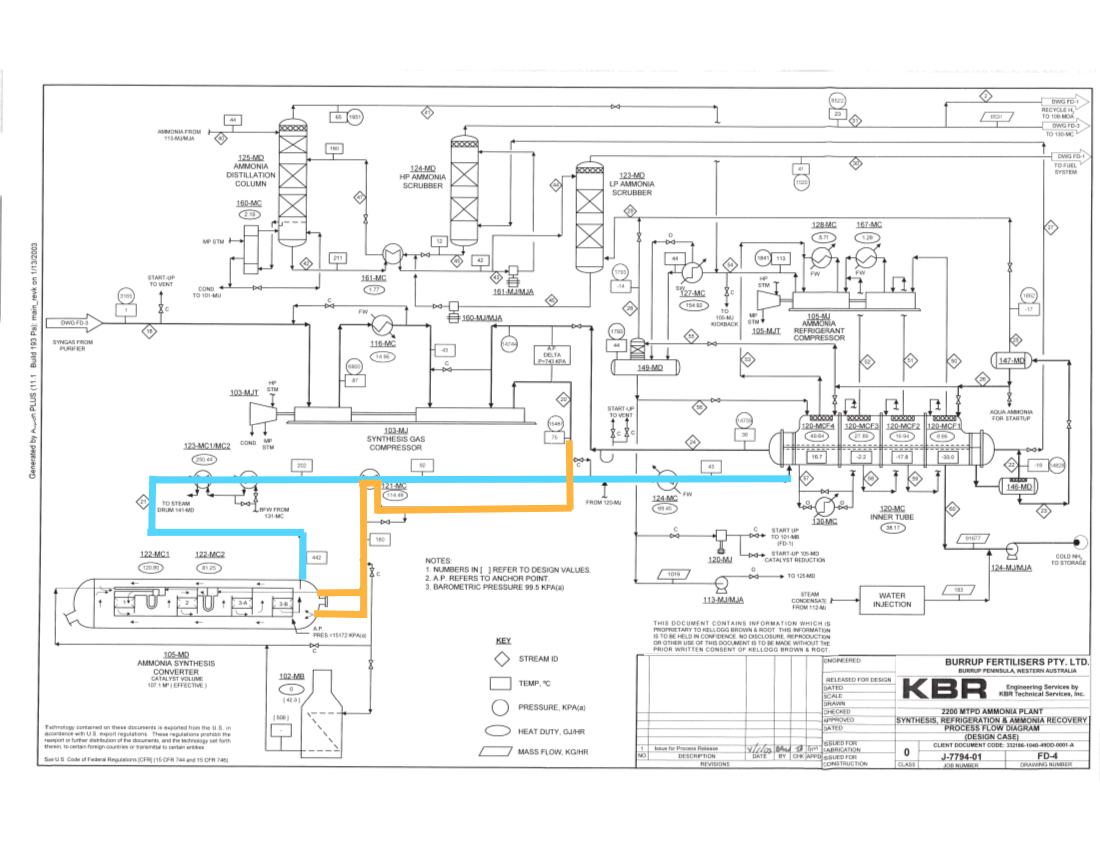
\includegraphics[scale=0.6]{task4/Plan1.png}
	\end{center}
	\caption{Circulation du flux}
	\label{cir1}
\end{figure}

\begin{figure}[h]
	\begin{center}
	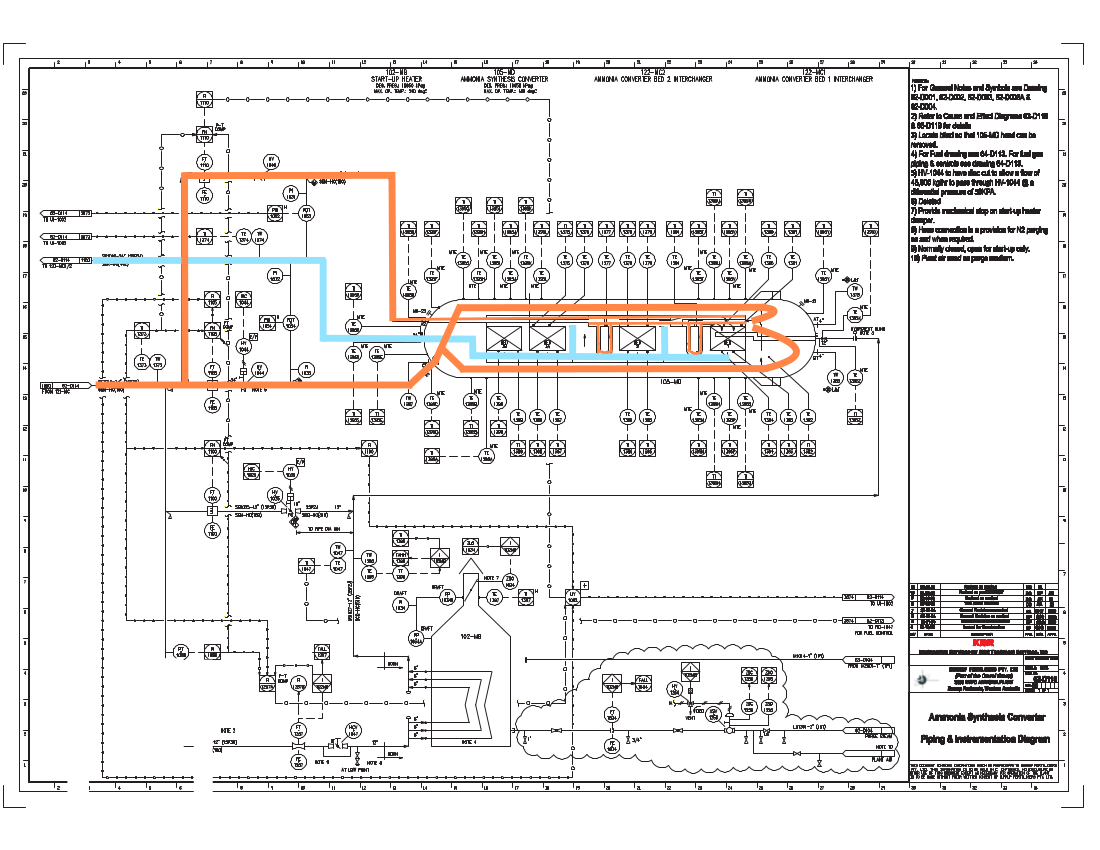
\includegraphics[scale=0.5]{task4/Plan2.png}
	\end{center}

	\caption{Circulation du flux}
	\label{cir2}
\end{figure}

\begin{figure}[h]
	\begin{center}
	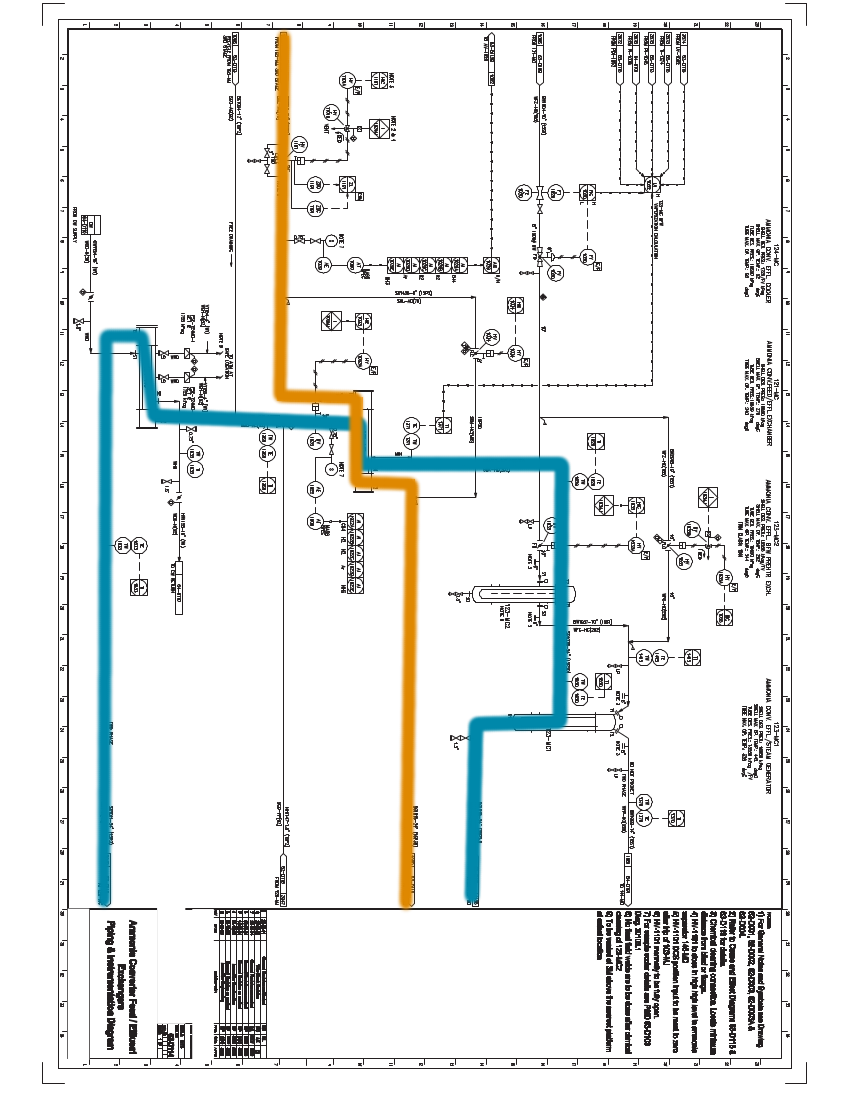
\includegraphics[scale=0.5]{task4/Plan2-2.png}
	\end{center}
	\caption{Circulation du flux}
	\label{cir3}
\end{figure}

\begin{figure}[h]
	\begin{center}
	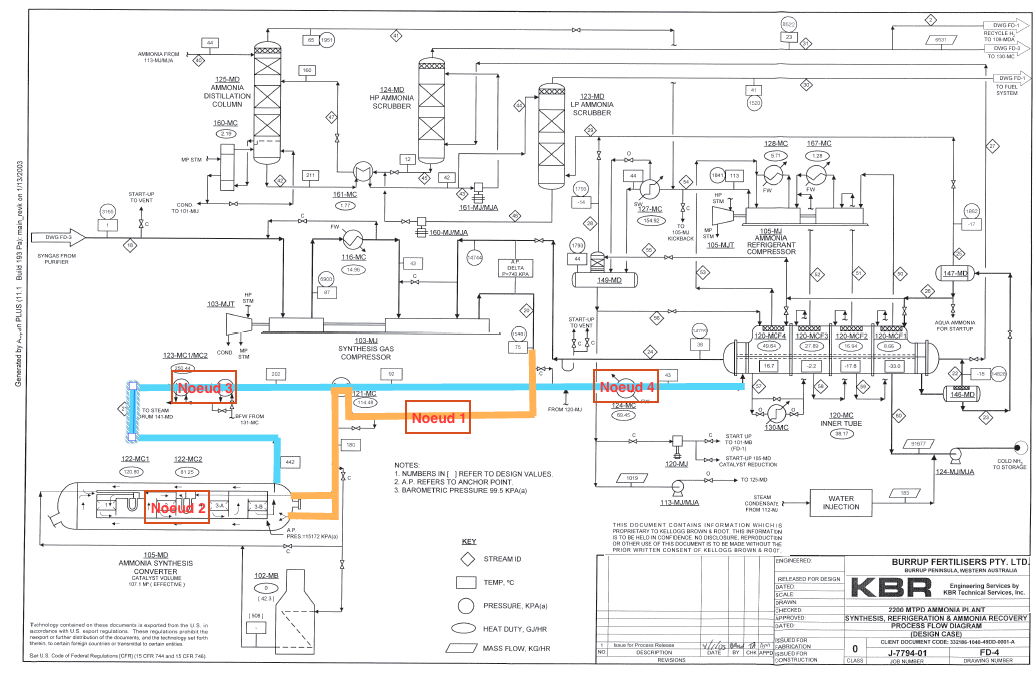
\includegraphics[scale=0.4]{task4/Position_des_differents_noeuds.png} 
	\end{center}
	\caption{Position des  Noeuds}
	\label{cir4}	
\end{figure}

\end{document}
